\chapter{Groene chemie en industriële processen}\label{ch:b3:green-industrial}

Ibuprofen werd vroeger gemaakt in zes stappen die meer massa weggooiden
dan ze behielden: aluminiumzouten, natriumchloride, ethanol, ammoniak en
azijnzuur verlieten de fabriek voor elke kilogram geneesmiddel. Sinds
1992 zet een katalytische route van drie stappen het grootste deel van de
atomen die ze gebruikt om in het product, en haar enige bijproduct,
azijnzuur, wordt teruggewonnen en verkocht. Dit hoofdstuk zet cijfers op
zulke vergelijkingen: \omterm{def:b3:green-industrial:atom-economy}{atoomeconomie}, \omterm{def:b3:green-industrial:e-factor}{E-factoren} en
\omterm{def:b3:green-industrial:pmi}{procesmassa-intensiteit}; daarna bekijkt het oplosmiddelen, energie en
\omterm{def:b3:green-industrial:lca}{levenscyclusanalyse}, hoe enkele van de grootste chemische processen
schoner gemaakt werden, en wat \omterm{def:b3:green-industrial:feedstock}{hernieuwbare grondstoffen} en \omterm{def:b3:complex-kinetics:enzyme}{enzymen}
veranderen.

\begin{recall}
Boek 1 voerde de \omterm{def:b3:green-industrial:atom-economy}{atoomeconomie} en de \omterm{def:b3:green-industrial:green-chemistry}{groene chemie} in; het deel van
jaar~1 rendementen; het deel van jaar~2 reactoren, omzetting,
selectiviteit, verblijftijd, omzetting per doorgang, recirculatie en
spui, adiabatische temperatuurstijging, elektrolysers en brandstofcellen.
\Cref{ch:b3:surfaces-catalysis} en
\cref{ch:b3:homogeneous-catalysis} behandelden de katalyse,
\cref{ch:b3:total-synthesis} de maatstaven van een syntheseroute.
\end{recall}

\begin{omfigure}
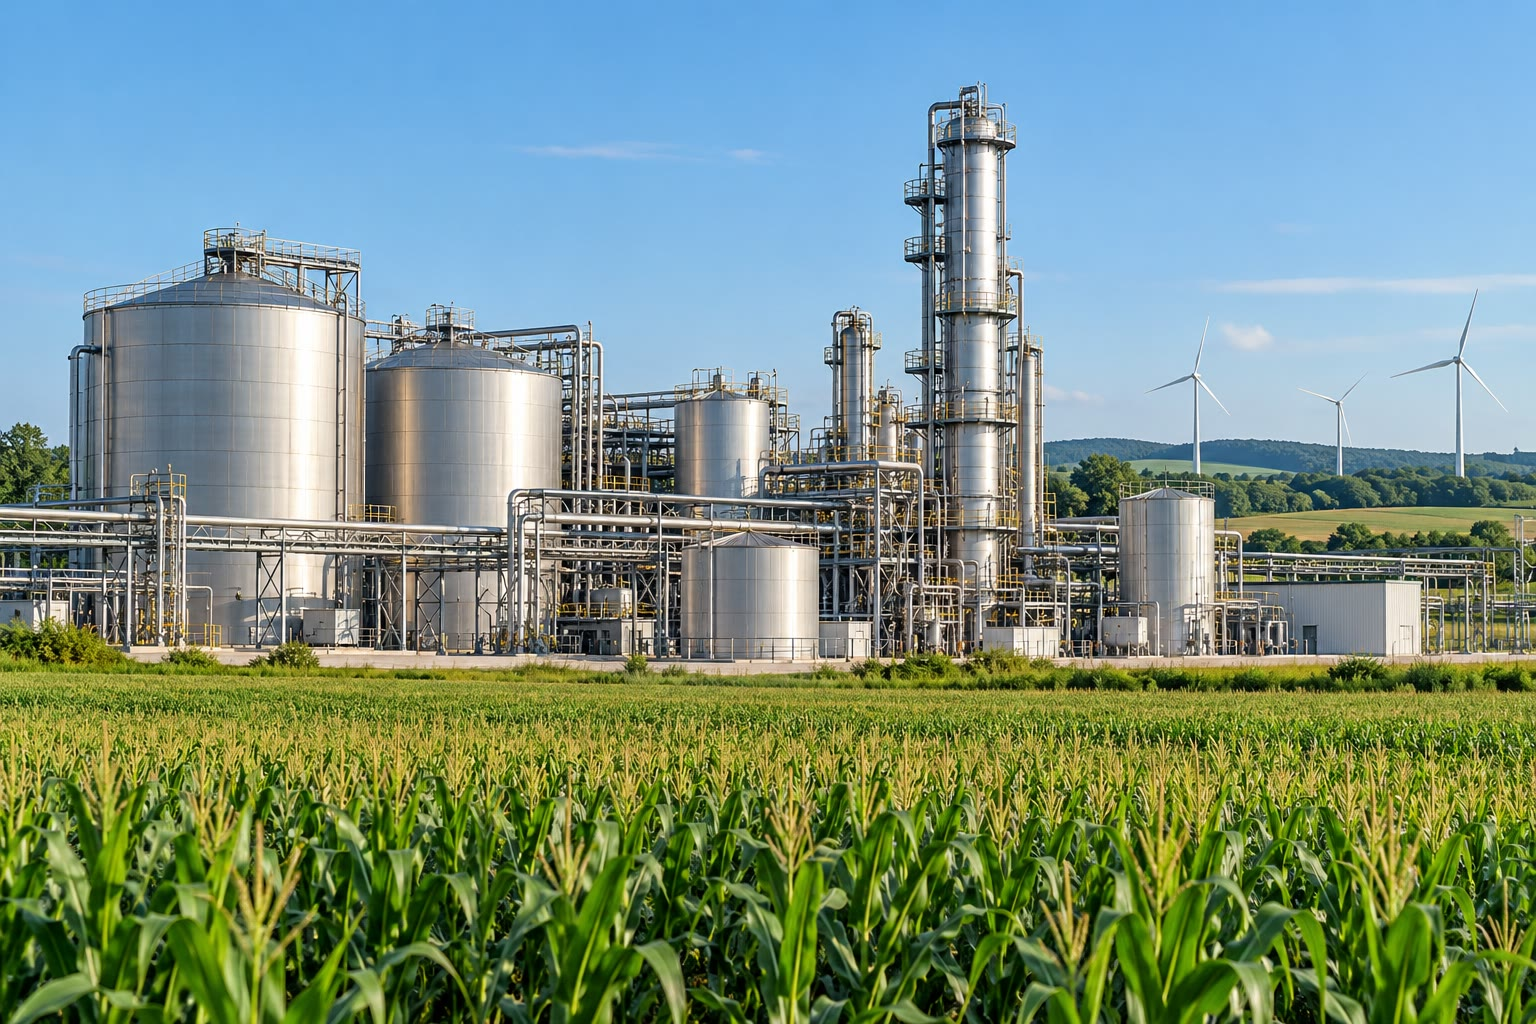
\includegraphics[width=0.58\linewidth]{images/book4/ai/b3-31-biorefinery.jpg}

{\small Een bioraffinaderij: fermentatietanks en een destillatiekolom die
gewassen en residuen omzetten in brandstoffen en
platformchemicaliën.}
\end{omfigure}

\section{Groenheid meten}

\begin{definition}[Groene chemie]\label{def:b3:green-industrial:green-chemistry}
\emph{Groene chemie}\index{groene chemie} is het ontwerpen van chemische
producten en processen die het gebruik en de vorming van gevaarlijke
stoffen beperken of uitsluiten, samengevat in twaalf principes: afval
voorkomen, de \omterm{def:b3:green-industrial:atom-economy}{atoomeconomie} maximaliseren, minder gevaarlijke stoffen
gebruiken en maken, veiligere producten ontwerpen, veiligere
oplosmiddelen gebruiken, energie besparen, \omterm{def:b3:green-industrial:feedstock}{hernieuwbare grondstoffen}
gebruiken, onnodige derivaten vermijden, katalysatoren verkiezen boven
stoichiometrische reagentia, ontwerpen voor afbraak, in real time
monitoren, en inherent veiligere chemie kiezen.
\end{definition}

\begin{definition}[Atoomeconomie]\label{def:b3:green-industrial:atom-economy}
De \emph{atoomeconomie}\index{atoomeconomie} van een reactie is de
molaire massa van het gewenste product gedeeld door de som van de molaire
massa's van alle beginstoffen in de kloppende vergelijking, uitgedrukt
als percentage.
\end{definition}

\begin{proposition}[Atoomeconomie per reactieklasse]\label{prop:b3:green-industrial:ae-classes}
Addities en omleggingen hebben een \omterm{def:b3:green-industrial:atom-economy}{atoomeconomie} van 100\,\%; substituties
en eliminaties minder.
\end{proposition}

\begin{proof}
Bij een additie, $\mathrm{A} + \mathrm{B} \to \mathrm{AB}$, of een omlegging, $\mathrm{A} \to \mathrm{A'}$, bevat het enige product alle
atomen van de beginstoffen, zodat zijn molaire massa gelijk is aan de som
van de hunne. Een
substitutie, $\mathrm{A{-}X} + \mathrm{Y} \to \mathrm{A{-}Y} + \mathrm{X}$, of een eliminatie, $\mathrm{A} \to \mathrm{B} + \mathrm{C}$, levert een
tweede product dat massa meeneemt.
\end{proof}

\begin{definition}[E-factor]\label{def:b3:green-industrial:e-factor}
De \emph{E-factor}\index{E-factor} van een proces is de massa afval per
massa product. In de volledige E-factor tellen alle inputs die niet in
het product terechtkomen als afval, oplosmiddelen en water inbegrepen; de
eenvoudige E-factor laat oplosmiddelen en water weg.
\end{definition}

\begin{definition}[Procesmassa-intensiteit]\label{def:b3:green-industrial:pmi}
De \emph{procesmassa-intensiteit}\index{procesmassa-intensiteit} (PMI) is
de totale massa materialen die in een proces gaan (beginstoffen,
reagentia, oplosmiddelen, water) per massa product.
\end{definition}

\begin{proposition}[PMI en E-factor]\label{prop:b3:green-industrial:pmi-e}
Voor dezelfde grens is $\mathrm{PMI} = E + 1$, met $E$ de volledige \omterm{def:b3:green-industrial:e-factor}{E-factor}.
\end{proposition}

\begin{proof}
Door behoud van massa verlaat alles wat erin gaat het proces als product
of als afval:
$m_{\mathrm{in}} = m_{\mathrm{product}} + m_{\mathrm{afval}}$. Delen door $m_{\mathrm{product}}$ geeft $\mathrm{PMI} = 1 + E$.
\end{proof}

\begin{definition}[Reactiemassa-efficiëntie]\label{def:b3:green-industrial:rme}
De \emph{reactiemassa-efficiëntie}\index{reactiemassa-efficientie@reactiemassa-efficiëntie}
(RME) van een reactie is de verkregen massa product gedeeld door de
totale massa van de gebruikte beginstoffen.
\end{definition}

\begin{proposition}[RME uit rendement en atoomeconomie]\label{prop:b3:green-industrial:rme}
$\mathrm{RME} = \mathrm{AE} \times \text{rendement}/\mathrm{SF}$, waarin de stoichiometrische factor $\mathrm{SF} \ge 1$ de massa van de
gebruikte beginstoffen is gedeeld door de massa die de kloppende
vergelijking vereist.
\end{proposition}

\begin{proof}
Voor één verwachte mol product vereist de vergelijking een massa $\sum M_r$ aan beginstoffen en
gebruikt de uitvoering $\mathrm{SF}\sum M_r$; ze geeft $\text{rendement} \times M_{\mathrm p}$ product. Delen geeft
$\mathrm{RME} = \text{rendement}\,M_{\mathrm p}/(\mathrm{SF}\sum M_r) = \mathrm{AE} \times \text{rendement}/\mathrm{SF}$.
\end{proof}

\begin{method}[De maatstaven van een route berekenen]\label{met:b3:green-industrial:metrics}
\begin{enumerate}
  \item Schrijf de kloppende vergelijking van elke stap op en bereken de
        \omterm{def:b3:green-industrial:atom-economy}{atoomeconomie} van de route uit alle beginstoffen die erin gaan.
  \item Tel uit het batchverslag de massa's op van alles wat ingebracht
        wordt (beginstoffen, reagentia, oplosmiddelen, water,
        opwerkingsmaterialen): PMI = totale invoer / product.
  \item $E = \mathrm{PMI} - 1$; trek teruggewonnen en hergebruikte stromen af als ze binnen de
        grens liggen, en vermeld dat.
  \item RME voor elke stap: product / beginstoffen, om te zien waar
        materiaal verloren gaat (laag rendement, overmaat reagens of slechte
        \omterm{def:b3:green-industrial:atom-economy}{atoomeconomie}).
\end{enumerate}
\end{method}

\begin{omfigure}
\begin{tikzpicture}
\begin{axis}[name=a, width=0.48\linewidth, height=5.4cm, ybar, bar width=14pt, ymin=0, ymax=110,
  xtick={1,2,3,4}, xticklabels={{ibuprofen, 6 stappen}, {ibuprofen, 3 stappen}, {EO, chloorhydrine}, {EO, direct}},
  x tick label style={font=\scriptsize, rotate=25, anchor=north east}, ylabel={atoomeconomie / \%},
  axis lines=left, tick label style={font=\scriptsize}, label style={font=\small},
  nodes near coords, nodes near coords style={font=\scriptsize, /pgf/number format/fixed, /pgf/number format/precision=0},
  enlarge x limits=0.18]
\addplot[fill=omMeth!55, draw=omMeth] table[x=i, y=AE] {figdata/out/bachelor-3-green-metrics.dat};
\end{axis}
\begin{axis}[at={(a.east)}, anchor=west, xshift=1.4cm, width=0.48\linewidth, height=5.4cm, ybar, bar width=14pt, ymin=0, ymax=3.4,
  xtick={1,2,3,4}, xticklabels={{ibuprofen, 6 stappen}, {ibuprofen, 3 stappen}, {EO, chloorhydrine}, {EO, direct}},
  x tick label style={font=\scriptsize, rotate=25, anchor=north east}, ylabel={minimale E-factor},
  axis lines=left, tick label style={font=\scriptsize}, label style={font=\small},
  nodes near coords, nodes near coords style={font=\scriptsize, /pgf/number format/fixed, /pgf/number format/precision=2},
  enlarge x limits=0.18]
\addplot[fill=omThm!45, draw=omThm] table[x=i, y=Emin] {figdata/out/bachelor-3-green-metrics.dat};
\end{axis}
\end{tikzpicture}

{\small Atoomeconomieën van twee routes naar ibuprofen en twee routes naar
ethyleenoxide (EO), en de kleinste \omterm{def:b3:green-industrial:e-factor}{E-factoren} die ze toelaten (alle
rendementen 100\,\%, geen oplosmiddel):
$E_{\min} = (1 - \mathrm{AE})/\mathrm{AE}$. Echte \omterm{def:b3:green-industrial:e-factor}{E-factoren}, met rendementen onder 100\,\%, overmaat reagentia en
oplosmiddelen, zijn groter.}
\end{omfigure}

\section{Oplosmiddelen en energie}

Oplosmiddelen vormen meestal het grootste deel van de massa van een
proces in de fijnchemie of de farmaceutische industrie. Gidsen voor de
keuze van oplosmiddelen rangschikken ze volgens criteria van veiligheid,
gezondheid en milieu: water, ethanol, ethylacetaat,
2-methyltetrahydrofuraan en anisool worden aanbevolen; dichloormethaan,
chloroform, benzeen, hexaan, dimethylformamide en 1,4-dioxaan moeten
vermeden of verboden worden. Water, superkritisch koolstofdioxide (dat
apolaire verbindingen oplost en geen residu achterlaat wanneer de druk
weggenomen wordt) en reacties zonder oplosmiddel pakken het probleem bij
de bron aan.

\begin{method}[Een gids voor oplosmiddelkeuze gebruiken]\label{met:b3:green-industrial:solvent-choice}
\begin{enumerate}
  \item Som op wat het oplosmiddel moet doen: de beginstoffen oplossen,
        de reagentia doorstaan, koken bij een bruikbare temperatuur, zich
        bij de opwerking van water scheiden.
  \item Kies eerst uit de aanbevolen klasse; controleer de
        gevarenaanduidingen.
  \item Als een problematisch oplosmiddel nodig is, zoek dan een
        aanbevolen oplosmiddel met dezelfde functie
        (2-methyltetrahydrofuraan voor dichloormethaan of THF bij
        extracties, ethylacetaat en heptaan voor hexaan in de
        chromatografie).
  \item Plan de terugwinning door destillatie, en tel wat verloren gaat
        mee in de \omterm{def:b3:green-industrial:e-factor}{E-factor}.
\end{enumerate}
\end{method}

\begin{definition}[Procesintensivering]\label{def:b3:green-industrial:intensification}
\emph{Procesintensivering}\index{procesintensivering} is het herontwerpen
van apparatuur en bedrijfsomstandigheden om een proces veel kleiner,
veiliger of efficiënter te maken: continue stroomreactoren met kleine
volumes en grote warmtewisselende oppervlakken, reactieve destillatie,
microgolfverwarming.
\end{definition}

In een stroomreactor bestaat op elk ogenblik maar een klein volume van
een gevaarlijk intermediair, en wordt warmte veel sneller afgevoerd dan
in een groot batchvat; reacties die in een tank op hol zouden slaan,
kunnen bij hogere temperaturen en concentraties uitgevoerd worden.
Katalysatoren vervangen stoichiometrische reagentia en besparen zowel het
reagens als het afval dat het wordt: de friedel-craftsacylering van de
oude ibuprofenroute gebruikte aluminiumchloride in stoichiometrische
hoeveelheid, die bij de opwerking vernietigd werd; de nieuwe gebruikt
waterstoffluoride als katalysator en oplosmiddel, dat teruggewonnen en
hergebruikt wordt.

\section{Denken in levenscycli}

\begin{definition}[Levenscyclusanalyse]\label{def:b3:green-industrial:lca}
Een \emph{levenscyclusanalyse}\index{levenscyclusanalyse} (LCA) evalueert
de milieueffecten van een product over zijn hele levensloop, van de
winning van grondstoffen tot de verwijdering. Ze wordt uitgedrukt per
\emph{functionele eenheid}\index{functionele eenheid}, de geleverde dienst
(bijvoorbeeld één wasbeurt van een lading wasgoed), binnen een
\emph{systeemgrens}\index{systeemgrens} die vermeldt welke processen
meegenomen worden. Een
\emph{analyse van wieg tot poort}\index{analyse van wieg tot poort}
stopt wanneer het product de fabriek verlaat.
\end{definition}

\begin{omfigure}
\begin{tikzpicture}[font=\scriptsize, >=Stealth,
  box/.style={draw, rounded corners, fill=omDef!10, align=center, minimum height=8mm, inner sep=3pt}]
  \node[box] (r) at (0,0) {winning van\\ grondstoffen};
  \node[box] (p) at (2.6,0) {chemische\\ productie};
  \node[box] (f) at (5.2,0) {formulering,\\ verpakking};
  \node[box] (u) at (7.8,0) {gebruik};
  \node[box] (e) at (10.2,0) {levenseinde:\\ recycling,\\ verwijdering};
  \foreach \a/\b in {r/p, p/f, f/u, u/e} \draw[->, thick] (\a) -- (\b);
  \draw[omThm, thick, dashed, rounded corners] (-1.1,-0.75) rectangle (3.75,0.75);
  \node[omThm, anchor=north] at (1.3,-0.8) {grens van wieg tot poort};
  \draw[omMeth, thick, dashed, rounded corners] (-1.25,-1.35) rectangle (11.5,0.95);
  \node[omMeth, anchor=north] at (5.1,-1.4) {grens van wieg tot graf};
  \node[anchor=south] at (5.1,1.0) {invoer: materialen, energie, water \quad uitvoer: product, emissies, afval};
\end{tikzpicture}

{\small Stadia van de levensloop van een product en twee systeemgrenzen.
Invoer en uitvoer worden geïnventariseerd voor elk proces binnen de
grens en omgerekend naar effectcategorieën (klimaatverandering,
verzuring, watergebruik, toxiciteit\dots) per
\omterm{def:b3:green-industrial:lca}{functionele eenheid}.}
\end{omfigure}

\begin{definition}[Koolstofvoetafdruk]\label{def:b3:green-industrial:carbon-footprint}
De \emph{koolstofvoetafdruk}\index{koolstofvoetafdruk} van een product is
zijn uitstoot van broeikasgassen over de levenscyclus, uitgedrukt als de
massa koolstofdioxide met hetzelfde opwarmend effect.
\end{definition}

\begin{method}[Een vergelijkende LCA opzetten]\label{met:b3:green-industrial:lca}
\begin{enumerate}
  \item Formuleer het doel en de \omterm{def:b3:green-industrial:lca}{functionele eenheid}: vergelijk wat
        dezelfde dienst levert, niet dezelfde massa.
  \item Trek voor beide opties dezelfde \omterm{def:b3:green-industrial:lca}{systeemgrens}.
  \item Inventariseer de invoer en uitvoer van elk proces erbinnen, met
        gegevensbronnen en data.
  \item Reken om naar effectcategorieën, zoek dan afwegingen (minder
        koolstof maar meer water) en test hoe gevoelig de conclusie is voor
        de gegevens.
\end{enumerate}
\end{method}

\section{Grote processen en hun verbetering}

\begin{proposition}[Koolstofdioxide uit ammoniak]\label{prop:b3:green-industrial:smr}
Ammoniak maken met waterstof uit de stoomreforming van methaan zet, alleen
al uit de grondstof, $3/8$ mol $\ce{CO2}$ per mol $\ce{NH3}$ vrij: ongeveer \qty{0.97}{t} $\ce{CO2}$ per ton ammoniak.
\end{proposition}

\begin{proof}
Reforming gevolgd door de watergasshiftreactie geeft in totaal $\ce{CH4 + 2H2O -> CO2 + 4H2}$. De synthese
is $\ce{N2 + 3H2 -> 2NH3}$: twee mol ammoniak vereist drie mol waterstof, d.w.z.\ $3/4$ mol
methaan en $3/4$ mol $\ce{CO2}$; per mol ammoniak $3/8$. Een ton ammoniak
(\qty{17.0}{g/mol}) is $\qty{5.88e4}{mol}$, wat $\qty{2.21e4}{mol} \times \qty{44.0}{g/mol} = \qty{0.97}{t}$ $\ce{CO2}$ geeft. Het verbranden van methaan
voor de warmte van de reforming voegt er nog aan toe.
\end{proof}

% ledger: nh3:world-2024
Ammoniakfabrieken, die zo'n 150 miljoen ton stikstof per jaar maken,
behoren tot de grootste afzonderlijke bronnen van industrieel
koolstofdioxide; waterstof uit elektrolyse met koolstofarme
elektriciteit, of koolstofafvang bij de reformer, zijn de wegen om die
uitstoot te verminderen. De ammoniaklus zelf, met haar lage omzetting
per doorgang, de recirculatie van niet-omgezet gas en de spui van het
argon en methaan die zich anders zouden ophopen, is al efficiënt.

\begin{omfigure}
\begin{tikzpicture}[font=\scriptsize, >=Stealth,
  box/.style={draw, rounded corners, fill=omMeth!10, align=center, minimum height=8mm, inner sep=3pt}]
  \node[box] (m) at (0,0) {menger};
  \node[box] (c) at (2.6,0) {compressor};
  \node[box] (r) at (5.2,0) {reactor\\ (ijzerkatalysator)};
  \node[box] (s) at (8.0,0) {condensor,\\ scheider};
  \draw[->, thick] (-1.8,0) -- (m) node[pos=0, left, align=right] {$\ce{N2 + 3H2}$\\ (aanvulling)};
  \draw[->, thick] (m) -- (c); \draw[->, thick] (c) -- (r); \draw[->, thick] (r) -- (s);
  \draw[->, thick] (s) -- ++(0,-1.2) node[below] {vloeibaar $\ce{NH3}$};
  \draw[->, thick] (s.north) -- ++(0,0.8) -| node[pos=0.25, above] {recirculatie van niet-omgezet gas} (m.north);
  \draw[->, thick, omThm] ($(s.north)+(0,0.8)$) -- ++(1.6,0) node[right] {spui (Ar, $\ce{CH4}$)};
\end{tikzpicture}

{\small De ammoniaksyntheselus: vers gas wordt gemengd met
gerecirculeerd gas, gecomprimeerd en over de katalysator geleid;
ammoniak wordt uitgecondenseerd, het niet-omgezette gas keert terug, en
een kleine spuistroom verwijdert de inerte gassen die zich anders zouden
ophopen.}
\end{omfigure}

Andere grote processen tonen dezelfde lessen. Het contactproces voor
zwavelzuur is zo exotherm dat een moderne fabriek stoom en elektriciteit
uitvoert. Ethyleenoxide werd eerst gemaakt via ethyleenchloorhydrine, met
calciumchloride als afval; de directe oxidatie van etheen met zuurstof op
zilver, een additie met een \omterm{def:b3:green-industrial:atom-economy}{atoomeconomie} van 100\,\%, verving die
route, ten koste van wat etheen dat tot koolstofdioxide verbrandt.
Propyleenoxide wordt nu ook gemaakt met waterstofperoxide op een
titaanzeolietkatalysator, met water als enig bijproduct. Adipinezuur,
gemaakt door oxidatie van cyclohexanol en cyclohexanon met salpeterzuur,
zet distikstofoxide vrij, een sterk broeikasgas, dat fabrieken nu
katalytisch vernietigen.

\section{Hernieuwbare grondstoffen en biokatalyse}

\begin{definition}[Hernieuwbare grondstoffen]\label{def:b3:green-industrial:feedstock}
Een \emph{hernieuwbare grondstof}\index{hernieuwbare grondstof} is een
grondstof die op een menselijke tijdschaal aangevuld wordt, zoals
plantaardige biomassa. Een
\emph{platformmolecuul}\index{platformmolecuul} is een eenvoudige
verbinding die er in grote hoeveelheden uit gemaakt wordt en in veel
producten omgezet: ethanol, melkzuur, barnsteenzuur, glycerol,
levulinezuur, furfural, 5-(hydroxymethyl)furfural.
\end{definition}

\begin{definition}[Biokatalyse]\label{def:b3:green-industrial:biocatalysis}
\emph{Biokatalyse}\index{biokatalyse} is het gebruik van \omterm{def:b3:complex-kinetics:enzyme}{enzymen},
geïsoleerd of in cellen, als katalysatoren voor chemische omzettingen.
\end{definition}

\omterm{def:b3:complex-kinetics:enzyme}{Enzymen} werken in water bij ongeveer kamertemperatuur met een
uitzonderlijke selectiviteit, en gerichte evolutie past ze nu aan
niet-natuurlijke substraten aan: een daartoe geëvolueerd transaminase
verving een door rodium gekatalyseerde asymmetrische hydrogenering bij de
productie van het diabetesmiddel sitagliptine, en ketoreductasen maken
veel chirale alcoholen. Koolstofdioxide zelf is een grondstof: ureum
wordt eruit gemaakt met ammoniak, en methanol met waterstof.
Polyethyleentereftalaat kan door glycolyse of methanolyse, of door
gemodificeerde \omterm{def:b3:complex-kinetics:enzyme}{enzymen}, tot zijn monomeren gedepolymeriseerd en opnieuw
gepolymeriseerd worden.

\begin{inthelab}[Dichloormethaan vervangen bij een opwerking]
Een product dat met dichloormethaan uit water geëxtraheerd werd, wordt in
plaats daarvan geëxtraheerd met 2-methyltetrahydrofuraan: het wordt uit
biomassa gemaakt, scheidt zich netjes van water (het is maar gedeeltelijk
mengbaar), en vormt de bovenste laag, niet de onderste, wat de volgorde
van de handelingen met de scheitrechter verandert. De organische lagen
worden gedroogd, het oplosmiddel wordt onder verlaagde druk afgedestilleerd
en voor hergebruik opgevangen.
\end{inthelab}

\begin{safety}{\ghs[0.62cm]{GHS02}\ghs[0.62cm]{GHS04}\ghs[0.62cm]{GHS06}\ghs[0.62cm]{GHS08}}
% ledger: ghs4:EO, ghs:CH2Cl2, ghs4:2MeTHF
Ethyleenoxide: zeer licht ontvlambaar gas onder druk, giftig bij
inademing, kan kanker en genetische defecten veroorzaken; het bestaat
alleen in gesloten industriële systemen en sterilisatie-eenheden.
Dichloormethaan is verdacht kankerverwekkend, en 2-methyltetrahydrofuraan
is ontvlambaar en bijtend voor de ogen: een groener oplosmiddel is geen
onschadelijk oplosmiddel.
\end{safety}

\begin{history}[Twaalf principes en één getal]
Paul Anastas en John Warner publiceerden de twaalf principes van de
\omterm{def:b3:green-industrial:green-chemistry}{groene chemie} in 1998. Roger Sheldon voerde de \omterm{def:b3:green-industrial:e-factor}{E-factor} in 1992 in, toen
hij opmerkte dat de fijnchemie en de farmaceutische industrie, hoewel
klein in tonnage, per kilogram product veel meer afval maakten dan de
bulkchemie. Het ibuprofenproces van drie stappen, gestart in 1992, werd
een van de vroege voorbeelden van de nieuwe aanpak.
\end{history}

\section{Oefeningen}

\begin{exercise}[$\star$]\label{exo:b3:green-industrial:1}
Bereken de \omterm{def:b3:green-industrial:atom-economy}{atoomeconomie} van de diels-alderreactie van butadieen met
etheen, van de verestering van azijnzuur met ethanol, en van de
wittigreactie van benzaldehyde met $\ce{Ph3P=CH2}$ (die styreen en trifenylfosfineoxide geeft).
\end{exercise}

\begin{exercise}[$\star$]\label{exo:b3:green-industrial:2}
Een batch gebruikt 120 kg materialen (beginstoffen, oplosmiddelen en
water) en geeft 8.0 kg product. Bereken de PMI en de volledige \omterm{def:b3:green-industrial:e-factor}{E-factor}.
\end{exercise}

\begin{exercise}[$\star$]\label{exo:b3:green-industrial:3}
Kies een \omterm{def:b3:green-industrial:lca}{functionele eenheid} om twee wasmiddelen te vergelijken, en zeg
waarom ``één kilogram poeder'' een slechte keuze zou zijn.
\end{exercise}

\begin{exercise}[$\star$]\label{exo:b3:green-industrial:4}
Stel groenere vervangers voor van dichloormethaan bij een extractie,
hexaan in de chromatografie, en DMF bij een amidekoppeling.
\end{exercise}

\begin{exercise}[$\star\star$]\label{exo:b3:green-industrial:5}
Een verestering van 60.0 g azijnzuur met 92.0 g ethanol (tweemaal de
stoichiometrische hoeveelheid) geeft 70.4 g ethylacetaat. Bereken het
rendement, de \omterm{def:b3:green-industrial:atom-economy}{atoomeconomie}, de stoichiometrische factor en de RME, en
controleer het verband ertussen.
\end{exercise}

\begin{exercise}[$\star\star$]\label{exo:b3:green-industrial:6}
Bereken de atoomeconomieën van de chloorhydrineroute en van de directe
oxidatie naar ethyleenoxide, en de massa calciumchloride die de eerste
per ton ethyleenoxide maakt.
\end{exercise}

\begin{exercise}[$\star\star$]\label{exo:b3:green-industrial:7}
Controleer de hoeveelheid $\ce{CO2}$ per ton ammoniak uit het hoofdstuk, en bereken de hoeveelheid $\ce{CO2}$ per ton
waterstof uit stoomreforming.
\end{exercise}

\begin{exercise}[$\star\star$]\label{exo:b3:green-industrial:8}
Bereken uit $\Delta_rG^\circ$ de minimale elektrische energie, in kWh, om één
kilogram waterstof te maken door elektrolyse van vloeibaar water bij \qty{25}{\celsius}, en de energie uit $\Delta_rH^\circ$.
\end{exercise}

\begin{exercise}[$\star\star$]\label{exo:b3:green-industrial:9}
Als er één mol $\ce{N2O}$ ontstaat per mol adipinezuur ($\ce{C6H10O4}$) en het aardopwarmingsvermogen
van $\ce{N2O}$ 273 is (gegevens van de oefening), bereken dan de hoeveelheid $\ce{N2O}$ en het $\ce{CO2}$-equivalent
per ton adipinezuur zonder reductiemaatregelen.
\end{exercise}

\begin{exercise}[$\star\star\star$]\label{exo:b3:green-industrial:10}
Toon aan dat voor een reeks stappen de totale RME niet het product is van
de RME's van de stappen als overmaat reagentia gerecycleerd worden, en
leg uit hoe recycling de \omterm{def:b3:green-industrial:e-factor}{E-factor} verandert.
\end{exercise}

\begin{exercise}[$\star\star\star$]\label{exo:b3:green-industrial:11}
Een procesverbetering verlaagt het oplosmiddel in een stap van 20 L tot
5 L per kilogram product (dichtheid van het oplosmiddel \qty{0.80}{kg/L}, voor en na 90\,\% teruggewonnen door destillatie; gegevens
van de oefening). Bereken de verandering van de volledige \omterm{def:b3:green-industrial:e-factor}{E-factor}.
\end{exercise}

\begin{exercise}[$\star\star\star$]\label{exo:b3:green-industrial:12}
Een biogebaseerde route naar een monomeer heeft een kleinere
\omterm{def:b3:green-industrial:carbon-footprint}{koolstofvoetafdruk} maar vereist meer land en water dan de
petrochemische route. Hoe zou een vergelijkende LCA dit voorstellen, en
wat zou je nodig hebben om tussen beide te beslissen?
\end{exercise}

\section{Probleem: ibuprofen, zes stappen of drie?}

\begin{problem}[{Weekendprobleem --- ibuprofen, zes stappen of drie: de
atoomeconomieën van de twee routes, hun E-factoren, de katalysatoren die
het verschil maken, en het afval dat in een jaar vermeden wordt}]
\label{pb:b3:green-industrial:1}
% ledger: aw:C, aw:H, aw:O, aw:Cl, aw:Na, aw:N
Gegevens van het probleem, per ton ibuprofen. Route van drie stappen:
0.71 t isobutylbenzeen, 0.55 t azijnzuuranhydride, 0.010 t waterstof,
0.14 t koolstofmonoxide, 0.05 t verliezen aan oplosmiddel en
katalysator; 0.31 t azijnzuur teruggewonnen en verkocht. Route van zes
stappen: 2.0 t reagentia en 1.5 t niet-teruggewonnen oplosmiddelen en
hulpstoffen. Een fabriek maakt 3000 t ibuprofen per jaar.

\medskip\noindent\textbf{Deel I --- \omterm{def:b3:green-industrial:atom-economy}{Atoomeconomie}.}
\begin{enumerate}
  \item Schrijf de drie stappen van de katalytische route op.
  \item Schrijf haar totaalvergelijking op.
  \item Bereken de betrokken molaire massa's en de \omterm{def:b3:green-industrial:atom-economy}{atoomeconomie}.
  \item Som de beginstoffen van de route van zes stappen op
        (friedel-craftsacylering, condensatie van Darzens met
        ethylchlooracetaat en natriumethoxide, hydrolyse en
        decarboxylering, vorming van het oxim, dehydratatie tot het
        nitril, hydrolyse).
  \item Bereken haar \omterm{def:b3:green-industrial:atom-economy}{atoomeconomie} uit de som van hun molaire massa's (met
        twee moleculen water).
  \item Welke bijproducten verlaten de oude route?
\end{enumerate}

\medskip\noindent\textbf{Deel II --- \omterm{def:b3:green-industrial:e-factor}{E-factoren}.}
\begin{enumerate}[resume]
  \item Bereken de massa die per ton product in de nieuwe route gaat.
  \item Bereken haar PMI en haar volledige \omterm{def:b3:green-industrial:e-factor}{E-factor}, met het azijnzuur
        als afval geteld.
  \item Bereken de \omterm{def:b3:green-industrial:e-factor}{E-factor} als het teruggewonnen azijnzuur als product
        geteld wordt.
  \item Bereken de PMI en de \omterm{def:b3:green-industrial:e-factor}{E-factor} van de oude route.
  \item Waarom is de echte \omterm{def:b3:green-industrial:e-factor}{E-factor} groter dan $(1 - \mathrm{AE})/\mathrm{AE}$?
  \item Welke van de twaalf principes illustreren de verschillen?
\end{enumerate}

\medskip\noindent\textbf{Deel III --- Katalysatoren.}
\begin{enumerate}[resume]
  \item Wat vervangt waterstoffluoride bij de acylering, en waarom is dat
        belangrijk?
  \item Wat katalyseert de hydrogenering van het keton tot de alcohol?
  \item Wat katalyseert de \omterm{def:b3:homogeneous-catalysis:carbonylation}{carbonylering} van de alcohol, en de chemie van
        welk hoofdstuk is dat?
  \item Waarom is azijnzuur in beide routes een bijproduct?
  \item Welke gevaren brengt de nieuwe route mee, en hoe worden ze
        beheerst?
  \item Waarom betekenen minder stappen ook minder energie?
\end{enumerate}

\medskip\noindent\textbf{Deel IV --- Een jaar.}
\begin{enumerate}[resume]
  \item Bereken het afval van de oude route voor de jaarproductie van de
        fabriek.
  \item Bereken dat van de nieuwe route (azijnzuur verkocht).
  \item Bereken het afval dat per jaar vermeden wordt.
  \item Is een lagere \omterm{def:b3:green-industrial:e-factor}{E-factor} altijd een kleinere milieu-impact?
  \item Wat zou een \omterm{def:b3:green-industrial:lca}{levenscyclusanalyse} toevoegen?
  \item Formuleer het resultaat: de \omterm{def:b3:green-industrial:atom-economy}{atoomeconomie} van de route van drie
        stappen.
\end{enumerate}
\end{problem}
